\scanpage{2}
$V$ : \uline{V.d. noethérien}, complet
\[
\operatorname{Spec}(V)\qquad k\ \text{\unsure{corps résid.}}\qquad K\ \text{\unsure{corps fractions}}
\]
\unsure{Groupe|Gpe} galoisien $(K)$

a) $\operatorname{car}(k)=0$\qquad \uuline{$k$ alg clos}
\figure{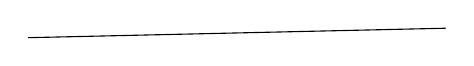
\begin{tikzpicture}\draw (0,0)--(5.3,.12);\end{tikzpicture}}
Les \unsure{extens|extensions} de $K$ sont \unsure{abél.} cycliques donc Kummeriennes.
\[
K^*/K^{*n}\simeq\mathbf Z/n\mathbf Z\qquad\text{(par la valuation)}
\]
Soit $\overline K$ clôture de $K$.
\diagram{\begin{tikzcd}[ampersand replacement=\&,column sep=small,row sep=small]
\Gamma(\overline K,K) \arrow[r,phantom,"\overset{\text{not}}{=}"] \& T_\infty(k) \arrow[r,phantom,"="] \& \displaystyle\varprojlim_n\underbrace{\mu_n(k)} \arrow[d,phantom,"\wr"] \& (\simeq\widehat{\mathbf Z})\\
\&\&\mathbf Z/n\mathbf Z
\end{tikzcd}}
\figure{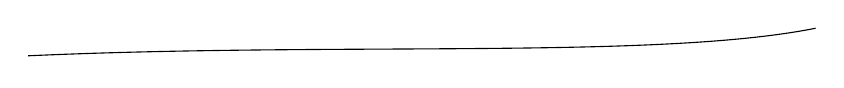
\begin{tikzpicture}\draw (0,0)..controls (4,.18) and (8,-.05)..(10,.35);\end{tikzpicture}}
Si $k$ car $\unsure{\ne0|p>0}$ $V$ pas \unsure{néces.} complet,
\[
\underset{\text{prem à }p}{\pi_1(K)}\longrightarrow\varprojlim_{n\text{ prem à }p}\mu_n(\unsure{k|K})
\]
\mspage{1}
